\begin{frame}
	\frametitle{Agent-based Framework}
	\begin{itemize}
		\item Cyclus is agent-based, which means it's very modular
		\item User can develop / plug in facilities
			\begin{itemize}
				\item User can `design' their own fuel cycle
				\item Highly customizable
			\end{itemize}
	\end{itemize}
	\begin{figure}[htbp!]
        \begin{center}
                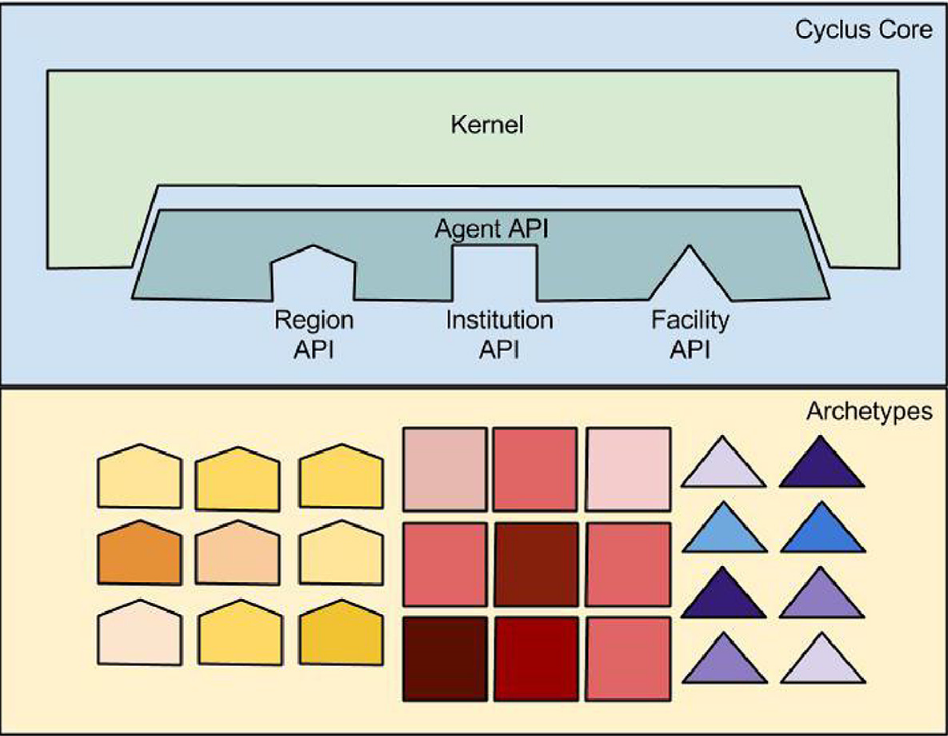
\includegraphics[width=.6\textwidth]{./images/cyclus_structure.png}
        \end{center}
        \caption{Modular Design of Cyclus}
        \label{fig:cyclus_struc}

	\end{figure}
\end{frame}

\begin{frame}
	\frametitle{General Info}
	\begin{itemize}
		\item Written in: C++, Python
		\item Input file: xml, json, python
		\item Output file: .sqlite, .hdf5
	\end{itemize}
\end{frame}


\begin{frame}
	\frametitle{Terminology}
	\begin{itemize}
		\item Archetypes: A collection of logic and behavior which can be configured into a prototype which can then be instantiated in simulation as a agent. Archetypes are represented as C++ classes that inherit from the base cyclus::Agent class. (e.g. Reactor module, Sink module)
		\item Prototypes: Archetype + parameters (e.g. Reactor with input-defined  \texttt{name, cycle time, assembly size, core size etc})
		\item Agents: Every single `entity' in play during simulation (Region, Institution, Facility)
	\end{itemize}
\end{frame}

\begin{frame}
	\frametitle{Terminology}
	\begin{itemize}
		\item Region: The group agent that is a collection of institutions (Can manage / control regions)
		\item Institution: Agent that manages facilities (Can deploy, decommission facilities)
		\item Facility: The agent that `trades' and does calculations (Trades material and transmutes, separates)
	\end{itemize}
\end{frame}

\begin{frame}
	\frametitle{Extensions - Archetypes}
	Since Cyclus is an extensible framework, anyone can develop a new archetype and plug-and-play. (\textcolor{blue}{Institution}, \textcolor{red}{region}, facility otherwise.)
	\begin{itemize}
		\item Cycamore: Sink, Storage, Recipe Reactor, Fuelfab, Enrichment, Source, \textcolor{blue}{DeployInst}, Mixer, Separations, \textcolor{red}{GrowthRegion}
		\item \textcolor{blue}{d3ploy}: Demand-driven deployment Institute (NEUP 16-10512)
		\item CYBORG: Reactor depletion analysis tool using ORIGEN
		\item Cyder: A cyclus disposal environment and repository object.
		\item CORRM: Continuous On-line Reprocessing Reactor Module.
		\item Pyre: Pyroprocessing module with non-proliferation metrics
		\item And more..
	\end{itemize}
\end{frame}

\begin{frame}
	\frametitle{Extensions - Analysis / Drivers}
	There are other tools to help visualization / output data management of Cyclus.
	\begin{itemize}
		\item RICKSHAW: Automated stochastic driver for Cyclus
		\item Cymetric: Extracts important fuel cycle metrics
		\item Analysis: Collection of functions to extract metrics (e.g. natU usage, trade between two facilities, etc.)
		\item Cymap(?): GIS visualization tool for Cyclus
		\item Cyclist: GUI for Cyclus (DEPRACATED)
	\end{itemize}
\end{frame}


\begin{frame}
	\frametitle{Installation - Binary}
	Better, more thorough explanations are in fuelcycle.org
	\begin{itemize}
		\item Windows: N/A
		\item MacOS: \texttt{conda install -c conda-forge cyclus cycamore}
		\item Linux: \texttt{conda install cyclus cycamore}
	\end{itemize}
\end{frame}


\begin{frame}
	\frametitle{Installation - Build from Source}
	\texttt{github.com/cyclus/cyclus} and \texttt{github.com/cycamore/cycamore} has the source files, and guides
	\begin{enumerate}
		\item Clone repository (\texttt{git clone [url]})
		\item Install dependency (see github guide README)
		\item \texttt{python install.py}
	\end{enumerate}
\end{frame}


\begin{frame}
	\frametitle{Installation - TroubleShooting}
	Installation difficulties? The Cyclus community is here. Look for your error message or make a new post.
	\begin{enumerate}
		\item Email jbae11@illinois.edu (me)
		\item Github Issue in \texttt{github.com/cyclus/cyclus}
		\item Cyclus google user group
	\end{enumerate}
\end{frame}

